\documentclass[../main.tex]{subfiles}
\begin{document}

\section{Notation \& Definitions}
In this section we introduce a mathematical description of the visualization pipeline where artist $A$ functions transform data of type $\Gamma(E)$ to an intermediate representation in prerendered display space of type $\Gamma(H)$:

\begin{equation}
    A: O(E) \rightarrow O(H)
    \label{eq:artist}
\end{equation}

\begin{equation}
    A: \tau \rightarrow \rho
\end{equation}

\begin{itemize}
\item $A$ is the function that converts an instance of data $\Gamma(E)$ to an instance of a visual representation $\Gamma(H)$ 
\item $E$ is a locally trivial fiber bundle over $K$ representing data space.
\item $K$ is a triangulizable space encoding the connectivity of the observations in the data. 
\item $H$ is a fiber bundle over $S$ representing visual space
\item $S$ is a simplacial complex of triangles encoding the connectivity of the visualization of the data in $E$
\item $\tau: K\rightarrow E$ is the data being visualized
\item $\rho: S \rightarrow H$ is the render map
\end{itemize}

When $E$ is a trivial fiber bundle $E = F \times K$, it can be assumed that all fibers $F_{k}$ over $k \in K$ are equal. Fiber bundles are product spaces of toplological spaces, which are a set of points with a set of neighborhoods for each point\cite{FiberBundle2020, rowlandFiberBundle}.

\subsection{Fiber Bundles}
We provide a brief introduction to fiber bundles because we model data, visual transformations, and a prerendered visual graphic as fiber bundles. A fiber bundle is a structure $(E, B, \pi, F)$  consisting of topological total space $E$, base space $K$, fiber space $F$ and the map from total space to base space:

\begin{equation}
    \begin{tikzcd}
        F \arrow[r, hook] & E \arrow[r, "\pi" description] & B  \\
    \end{tikzcd}
\end{equation}

where there is a bijection from $F$ to every fiber $F_b$ over point $b \in B$ in $E$ and the function $\pi: E \rightarrow B$ is the map into the $B$ quotient space of $E$.

\subsubsection{Base space}
\begin{figure}[ht]
    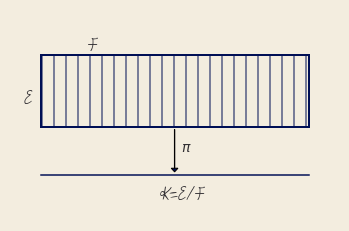
\includegraphics[width=0.4\linewidth]{figures/sections/math/k_qspace.png}
    \label{fig:kquote}
\end{figure}

$B$ is the quotient space of $E$, meaning it is the set of equivalence classes of elements $p$ in $E$ defined via the map $\pi: E \rightarrow B$ that sends each $p \in E$ to its equivalence class in $[p] \in B$ \cite{QuotientSpaceTopology2020,QuotientSpaceTopology2020}.

As shown in figure~\ref{fig:kquote}, the fibers $F$ divide $E$ into smaller spaces consisisting of $F$ and an open set neighborhood around $F$. This subdivision is projected down to the toplology $\mathcal{T}$

\begin{equation}
\mathcal{T}_b = \{U\subseteqq B: \{p \in E: [p] \in U\}\in \mathcal{T}_E\}
\end{equation}

where $[p] \in U$ is the point $b \in B$ with an open set surrounding it that has an open preimage in $E$ under the surjective map $\pi: p \rightarrow [p]$. 

\subsubsection{Fiber}
Every point in the base space $b \in B$ has a local open set neighborhood $U$ \cite{FiberBundle2020, rowlandFiberBundle}

\begin{equation}
    \begin{tikzcd}
        \pi^{-1}(U) \arrow[r, "\varphi" description] \arrow[d, "\pi" description] & U \times F \arrow[ld, "\mathrm{proj}_U"] \\
        U                                                                         &                                         
    \end{tikzcd}
    \label{eq:local_trivial}
\end{equation}
such that $\varphi: \pi^{-1}(U) \rightarrow U \times F$ is a homeomorphism where $\pi$ and $\mathrm{proj}_U$ both map to $U$ and the fiber over $k$ $F_b = \pi^{-1}({b \in B}) $ is homomorphic to the fiber $F$.

The section $f$ is the mapping from base space to total space $f: B\rightarrow E$ 
\begin{equation}
    \begin{tikzcd}
        F \arrow[r, hook] & E \arrow[d, "\pi" description]    \\
                          & B \arrow[u, "f" description, bend right]
        \end{tikzcd}
\end{equation}

such that it is the right inverse of $\pi$
\begin{equation}
    \pi(f(b)) = b \text{ for all } b \in B 
\end{equation}

In a locally trivial fiber bundle, $E = B \times F$ \cite{rowlandFiberBundle,FiberBundle2020}:
\begin{equation}
f(b) = (b, g(b))
\end{equation}

where the domain of $g(b)$ is $F_b$ and returns a point $p$ in $F_b$. The space of all possible sections $f$ of $E$ is $\Gamma(E)$. All sections $f \in \Gamma(E)$ have the same fibers $F$ and connectivity $B$. 

\subsubsection{Sheaf and Stalk}
As described in equation~\ref{eq:local_trivial}, there is a local space $U \subset B$ around every $b$. The inclusion map $\iota: U \rightarrow B$ can be pulled back such that $\iota^{*}E$ is the space of $E$ restricted over $U$. 
\begin{equation}
    \begin{tikzcd}
        \iota^*E \arrow[d, "\pi"']           & E \arrow[d, "\pi"'] \arrow[l, "\iota^*" description]                    \\
        U \arrow[u, "\iota^*f"', bend right] & B \arrow[u, "f" description, bend right] \arrow[l, "\iota" description]
        \end{tikzcd}
\end{equation}

The localized section of fibers $\iota^*\f: U \rightarrow \iota^*E$ is the sheaf $O(E)$ with germ of $\xi^*f$. The neighborhood of points the sheaf lies over is the stalk $\mathscr{F}_b$ \cite{StalkSheaf2019,spanier1989algebraic}

\begin{equation}
    \iota^{-1}\mathscr{F}(\{b\}) = \varinjlim_{b\subseteq U}\mathscr{F}(U) =  \varinjlim_{b \in U} = \mathscr{F}_b 
\end{equation}

which through $\iota$ gets the data in $E$ at and near to $b$. Restricting the artist to the sheaf means the artist knows the data in $F$ and also has access to derivatives of the data. This property is useful for some visual transformations. 
%% gives all direvatives but we need the jet which is Add stuff about jets

\subsection{Data Model}

We use a fiber bundle model to represent the data, as proposed by Butler.  
\cite{butlerVectorBundleClassesForm1992,butlerVisualizationModelBased1989}.
\begin{figure}[ht]
    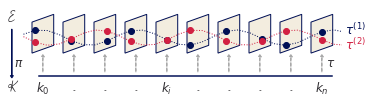
\includegraphics[width=.2\linewidth]{figures/sections/math/fiberbundle.png}
    \caption{write up some words here}
    \label{fig:fiberbundle}
\end{figure}

As illustrated by figure~\ref{fig:fiberbundle}, the vertical lines $F$ are the range of possible temperature values embedded in the total space $E$. The base space $K$ of the fiber bundle is a line because the data points $r$ in $E$ are on a space that is  continous in one dimension. 

\subsubsection{Base Space $K$}


\begin{figure}[ht]
    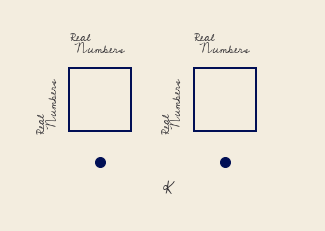
\includegraphics[width=0.2\linewidth]{figures/sections/math/temp_1k.png}
    %% add box around neighboring P and Map
    \label{fig:k_data}
\end{figure}

\begin{figure}[ht]
    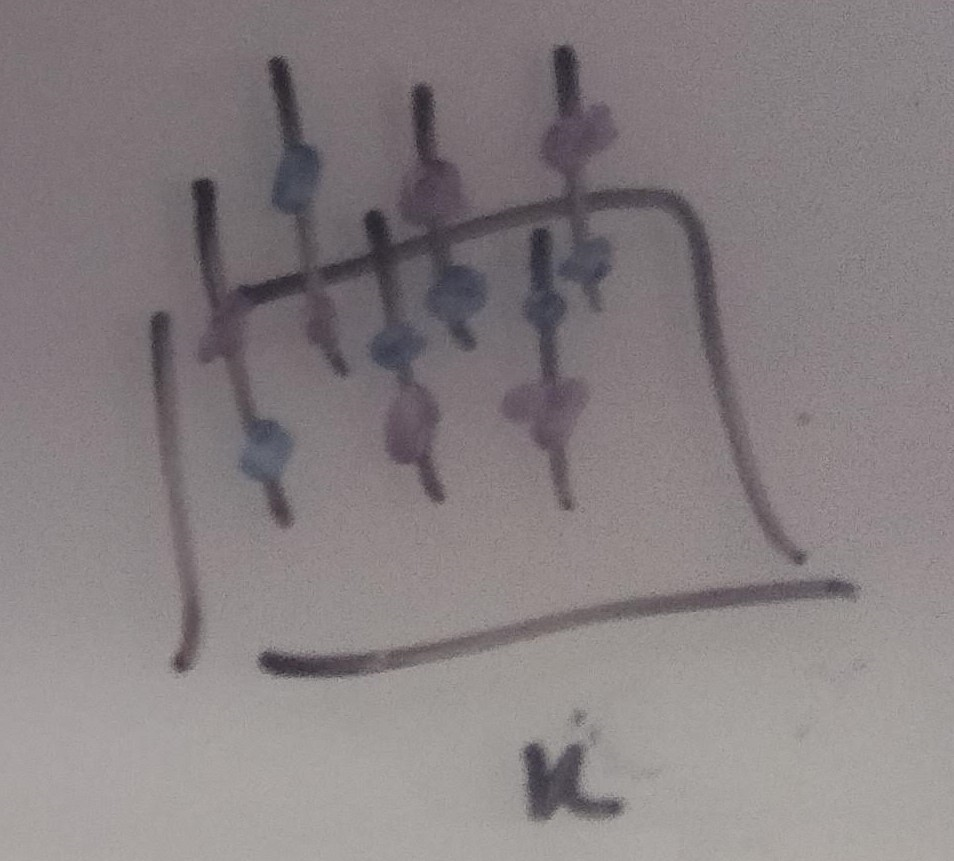
\includegraphics[width=0.2\linewidth]{figures/sections/math/temp_2k.png}
\end{figure}

in figure~\ref{fig:k_data}, temperature is the only one data field in $r$ but the $K$ base spaces are different. subfig[1] is a timeseries, so the temperature in $r$ at time $t$ is dependent on the temperature in $r_{t-1}$ and the temperature in $r_{t+1}$ is dependent on  $r_t$; this connectivity is expressed as a one dimensional $K$ where $K$ is the number line. In the case of the map, every temperature in $r$ is dependent on its nearest neighbors on the plane, and one way to express this is by encoding $K$ as a plane. $K$ does not know the time or latitude or longitude of the point as those are metadata variables describing the $k$ rather than the value of $k$. The mapping $\tau: K \rightarrow E$ provides the binding between the key $k \in K$ and the value $r$ in $E$ \cite{munznerChDataAbstraction}.

\subsubsection{Fiber Space $F$}
We use Spivak's formalization of data base schemas as the basis of our fiber space $F$ \cite{spivakSIMPLICIALDATABASES}. He defines the type specification 
\begin{equation}
\pi: U \rightarrow DT
\end{equation}

where $DT$ is the set of data types (as identified by their names) and $U$ is the disjoint set of all possible objects $x$ of all types in $DT$. This means that for each type $T\in DT$, the preimage $\pi^{-1}(T)\subset U $ is the domain of $T$, and $x \in \pi^{1}(T)\subset U$ is an object of type $T$. Spivak then defines a schema $(C, \sigma)$ of type $\pi$, where $\pi$ is the universe of all types, such that 
\begin{equation}
\sigma: C \rightarrow DT
\end{equation}
where $C$ is the finite set of names of columuns, which we generalize to data fields in $E$. The set of all values restricted to the datatypes in $DT$ is $U_{\sigma}$

\begin{equation}
    \begin{tikzcd}
            U_{\sigma} \arrow[d, "\pi_{\sigma}" description] \arrow[r] & U \arrow[d, "\pi" description] \\
            C \arrow[r, "\sigma" description]                          & DT                            
    \end{tikzcd}
\end{equation}
The pullback $U_{\sigma} \coloneqq \sigma^{-1}(U)$ restricts $U$ to the datatypes of the fields in $C$ such that $U_{\sigma}$ is the fiber product $U \times_{DT} C$, and the pullback $\pi_{\sigma}:U_{\sigma} \rightarrow C$ specifies the domain bundle $U_{\sigma}$ over $C$ induced by $\sigma$. The fiber $F$ is the cartesian product of all sets in the disjoint union $U_{\sigma}$. 

For each field $c \in C$, the record function $r: C \rightarrow U_{\sigma}$ returns an object of type $\sigma(c) \in DT$. The set of all records $\Gamma(\sigma)$ is the set of all sections on $U_\sigma$. Spivak defines the $\tau$ mapping from an index of databases $K$ to records $\Gamma(\sigma)$ as $\tau: K \rightarrow \Gamma(\sigma)$. This is equivalent to $\tau: k \rightarrow E$ since $F = \Gamma(\sigma)$ and $F$ is the embedding in $E$ on which the records $r$ lie.
 

\begin{figure}[ht]
    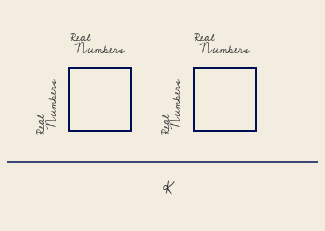
\includegraphics[width=0.2\linewidth]{figures/sections/math/temp_2f.png}
    \label{fig:}
\end{figure}
\begin{figure}[ht]
    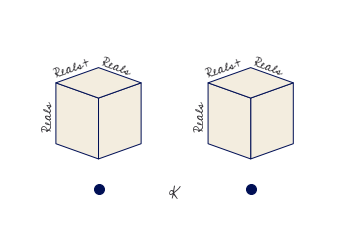
\includegraphics[width=0.2\linewidth]{figures/sections/math/temp_3f.png}
\end{figure}


%% pull out measurement
The fiber in figure~\ref{fig:temp} is the space of possible temperature values in degrees celsius, such that $F=[temp_{min}, temp_{max}]$ and is named \textrm{Temp}. In figure~\ref{fig:temp_time} \textrm{time} is encoded as a second dimension. This means that the set of possible values $F$ with $C=\{\textrm{Temp}, \textrm{Time}\}$:

\begin{equation}
F = [temp_{min}, temp_{max}] \times [time_{min}, time_{max}]
\end{equation}

and the function $\tau$ that retrieves records from $F$ is

\begin{align}
\tau(k) =(k, (r: \textrm{Temp}\rightarrow &temp, r: \textrm{Time}\rightarrow time))\\
&temp \in [temp_{min}, temp_{max}], time \in [time_{min}, time_{max}])
\end{align}

Since $\tau(k)=(k, r)$, $temp$ is bound to a named data field and $sigma$ binds $temp$ to a temperature data type. 



\subsection{Prerender Space}
\label{sec:display}

Every point $k \in K$ maps to a space $S_{k} \in S$, which is the topology of the output of the artist $A$. The space $H$ is a total space representing the predisplay space, with a fiber dependent on the render space and a base space of $\S$:
\begin{equation}
    \begin{tikzcd}
        D \arrow[r, hook] & H \arrow[d, "\pi" description, bend right] \\
                                    & S \arrow[u, "\rho" description, bend right] 
    \end{tikzcd}
\end{equation}

where $\rho: S \rightarrow H$ is mapping from a region $s$ on a mathematical encoding of the image to a region $xy$ on the screen that the renderer then maps to pixel space. For a physical screen display, the predisplay space is a trivial fiber bundle $H=\mathbb{R}^{7}\times S$ such that $\rho$ is
\begin{equation}
    \rho(s)  = \{x, y, z, g, b, a\}
    \label{eq:rho}
\end{equation}

To draw an image, a region, $H$ is inverse mapped into a region $s \in S$ where
\begin{equation}
s = \rho^{-1}_{XY}(xy)
\end{equation}
such that the rest of the fields in $\mathbb{R}^{7}$ are then integrated over $s$ to yield the remaining fields in $p$
%%change the integral to a double integral
\begin{align}
    R(p) &= \iint_s \rho_R(s)ds^{2}\\
    G(p) &= \iint_s \rho_G(s)ds^{2}\\
    B(p) &= \iint_s \rho_B(s)ds^{2}
\end{align}

Here we assume a single opaque 2D image such that the $z$ and $alpha$ fields can be omitted. 

\begin{figure}[h]
    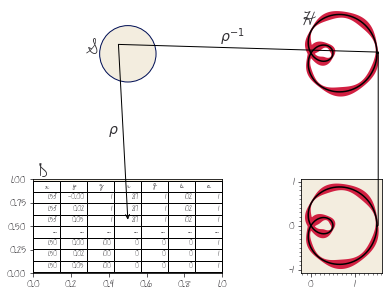
\includegraphics[width=.4\linewidth]{figures/sections/math/render.png}
    \caption{}
    \label{fig:render}
\end{figure}

As illustrated in figure~\ref{fig:render}, words.

\subsection{Artist}

The artist is a mapping from the sheaf $O(E)$ representing the data to a pre-render space $O(H)$. 
\begin{equation}
    A: O(E) \rightarrow O(H)
\end{equation}
The artist is composed of two stages, data $E$ to visual mappings $V$ and $V$ mappings composited to a visual in prerender space $H$:
\begin{equation}
insert triangle here
\end{equation}

The first stage of the artist $F: E \rightarrow V$ maps from data space to visual variable  \cite{carpendaleVisualRepresentationSemiology,bertinIIPropertiesGraphic2011,munznerWhatDataAbstraction2014} space
%%include the $
\begin{equation}
    \begin{tikzcd}
        E \arrow[r, "\nu" description]                                & V \\
        K \arrow[u, "\tau" description] \arrow[ru, "\mu" description] &  
    \end{tikzcd}
\end{equation}

such that $\nu: \tau \mapsto \mu$ is a homorphism where $\tau$ and $\mu$ are equivariant such that the properties of the field type persist in the visual representation. The map $\xi: S \rightarrow K$ goes from a region $s$ to it associated $k$ %%remove the taus from the diagram
\begin{equation}
    \begin{tikzcd}
        E \arrow[d, "\pi" description]              & H \arrow[d, "\pi" description]                                    \\
        K \arrow[u, "\tau" description, bend right] & S \arrow[l, "\xi" description] \arrow[lu, "\xi^*\tau" description]
        \end{tikzcd}
\end{equation}
such that when $\xi(s) = k$, there is a mapping from screen space to k  $\xi^*\tau(s) = \tau(k)$. The visual fiber bundle $V$ gets pulled back over $S$ via $\xi$ such that 
\begin{equation}
    \begin{tikzcd}
        \xi^*V \arrow[r, "q"']                      & H \\
        S \arrow[u, "\xi^*\mu"] \arrow[ru, "\rho"'] &  
        \end{tikzcd}
\end{equation}
the composition $q \circ \xi^*\mu$ generates the $\rho$ function described in section~\ref{sec:display}. 

An artist is the choice of ..... constraints are maps that preserve
\subsubsection{Compositing}

$Q$ is the assembly function for the visual idiom step something something something something something 

\subsubsection{Channels}
Each $\nu$ function maps a field $\tau_c$ to a paramterized visual field $\mu$, for example the color or shape visual channels \cite{bertinIIPropertiesGraphic2011,munznerMarksChannels}. The set of $\nu$ is a functor from data to visual space such that any $\nu$ is an equivariant map if 

\begin{equation}
    \begin{tikzcd}
        E_1 \arrow[r, "F" description] \arrow[d, "" description] & V_1 \arrow[d, "f" description] \\
        E_2 \arrow[r, "F" description]                            & V_2                           
    \end{tikzcd}
\end{equation}

$E$ or $J(E)$
%nu is functor
% examples of nu \tau\mu pairs - ordinal
%maybe param is the wrong thing 
Define a channel in terms of nus
This is what we mean by equivariance: 
step thrpoughh measurment scale groups
doesn't matter where computation lives

Here is the thing you need to preserve for {X} when writing a transform:


compose $\nu_{param}$ visual characteristic mappers
\begin{equation}
    \nu(\tau) = \mu
\end{equation}
where $\tau_{param}$ is a field in $\tau$ bound to the paremeter and $\mu_param$ is an intermediate visual representation such that $\nu_shape(\tau_shape)$ returns a $\mu_shape$ function that returns a shape for each $k$.

%For example, given a categorical field $c$ carry through temperature, maybe picture? 

$\nu$ is Hom set? 
1) must have identity
2) is composable
3) associativity 

homomorphism in land of categories:
objects in C, objects in D
C arrow D
 A-B for example stephens group scale

every $\nu$ is a functor that

put all the functorial things together is still functorial 
%argument into  is $\[\nu_{0}(\tau_{0}), \ldots \nu_{n}(\tau_{n})\]$








% complex columns are combined to \nu 


%% \nu is structure preserving if  E->E  & H->H under nu. \phi can be one of the scales in Stevens

% concrete example of \nu as one of our encodings, if artist is faithfully preserving 
% if was fiber, trans on fiber bundle. we require that nu goes to visual side that can support same translation  - work through some examples : if an artist wanted to preserve, this is what it would have to do - for example relations, interval





%%The measurement spaces $X$ are each variables and have the properties of measurement scales, such as Steven's nominal, ordinal, interval, and ratio \cite{stevensTheoryScalesMeasurement1946}. Stevens talks about measurements and this is how we define it here:.... can check symmatry under stevens via carry through on tau

 Can in theory approximate hatching/dashing/etc can be approximated w/ functions and neighborhood of k. 


\end{document}